\documentclass{beamer}

\usepackage[utf8]{inputenc}
\usepackage[spanish]{babel}
\usepackage{amsmath}
\usepackage{amssymb}
\usepackage{tikz}
\usetikzlibrary{arrows,calc,positioning}
\usetheme{Goddard}
\hypersetup{colorlinks,allcolors=.,urlcolor=magenta}

\title{Investigación de Operaciones II}
\subtitle{Unidad 3: Fundamentos de la Teoría de Colas}
\author{Ricardo Jesús Largaespada Fernández}
\institute{Ingeniería de Sistemas, DACTIC, UNI}
\date{05 de Mayo, 2025}

\begin{document}

% ---------------------------------------------------------------
% TÍTULO Y AGENDA
% ---------------------------------------------------------------
\frame{\titlepage}

\begin{frame}{Agenda}
    \tableofcontents
\end{frame}

\section{Sesión 16}

\begin{frame}{Sesión 16}
\textbf{Tema:}
\begin{enumerate}
    \item Estructura Básica de un modelo de colas.
    \begin{enumerate}
\item Proceso Básico de Cola
\item Disciplina de la Cola
\item Mecanismo de Servicio
\item Terminología y Notación.
\end{enumerate}
    \item Ejemplos de Sistemas de Colas Reales.
\end{enumerate}

\textbf{Objetivo:}
\begin{itemize}
    \item Identificar y caracterizar los componentes esenciales de un sistema de colas (proceso de llegada, disciplina de atención, mecanismo de servicio y notación estándar), relacionando su funcionamiento con situaciones prácticas en sistemas de servicio.
\end{itemize}
\end{frame}

\subsection{Introducción}
\begin{frame}{Introducción}
    \begin{itemize}
        \item Las colas son fenómenos omnipresentes en servicios y producción.
        \item El análisis de colas permite modelar tiempos de espera, optimizar recursos y mejorar la eficiencia.
        \item Aplicaciones en bancos, hospitales, centros de llamadas, manufactura, logística, entre otros.
    \end{itemize}
\end{frame}

\subsection{Estructura básica}
\begin{frame}{Estructura básica de un sistema de colas}
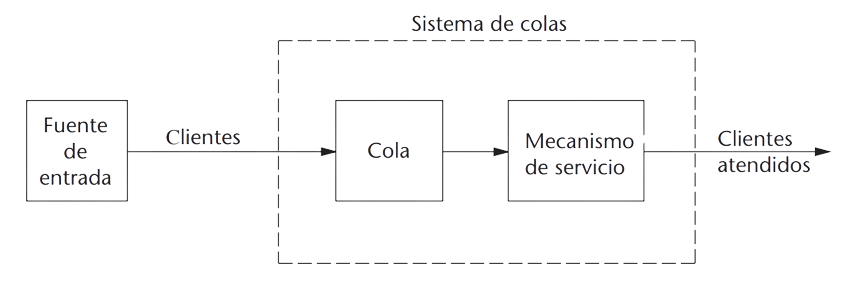
\includegraphics[width=0.9\linewidth]{images/cola_basica.png} % Puedes agregar esta imagen a tu directorio
\vspace{0.3cm}
\begin{itemize}
    \item \textbf{Fuente de entrada:} clientes que requieren servicio.
    \item \textbf{Cola:} donde esperan los clientes.
    \item \textbf{Disciplina:} orden en que son atendidos.
    \item \textbf{Servidor:} entidad que presta el servicio.
\end{itemize}
\end{frame}

\subsection{Proceso de cola}
\begin{frame}{Proceso básico de una cola}
    \begin{enumerate}
        \item Llegadas al sistema (frecuentemente modeladas con distribución de Poisson).
        \item Entrada en la cola (si el servidor está ocupado).
        \item Asignación de servidor según la disciplina establecida.
        \item Recepción del servicio (distribución exponencial o arbitraria).
        \item Salida del sistema.
    \end{enumerate}
\end{frame}

\subsection{Disciplina de cola}
\begin{frame}{Disciplina de la cola}
\begin{itemize}
    \item \textbf{FCFS (First Come, First Served):} el más común, justo y simple.
    \item \textbf{LCFS:} último en entrar, primero en salir (casos urgentes).
    \item \textbf{SIRO:} orden aleatorio.
    \item \textbf{Prioridad:} con base en urgencia o tipo de cliente.
\end{itemize}
\vspace{0.3cm}
Ejemplo: Whole Foods Market implementó una línea serpentina con disciplina FCFS para mejorar la satisfacción del cliente (Anderson).
\end{frame}

\subsection{Mecanismo de servicio}
\begin{frame}{Mecanismo de servicio}
    \begin{itemize}
        \item Puede ser una o múltiples estaciones (servidores).
        \item Servidores paralelos, en serie o en red.
        \item Tiempos de servicio comunes: exponenciales, Erlang, degenerados.
    \end{itemize}
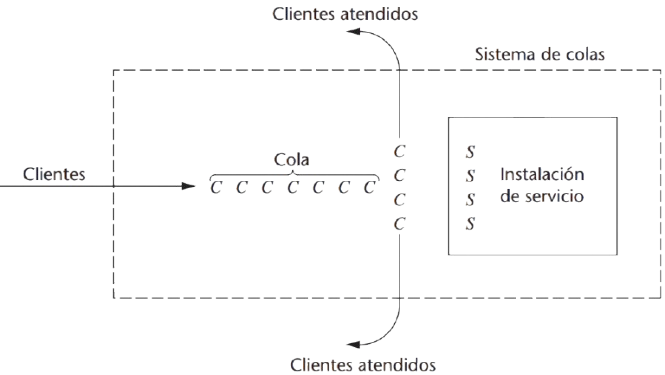
\includegraphics[width=0.8\linewidth]{images/servidores.png}
\end{frame}

\subsection{Terminología y notación}
\begin{frame}{Notación y métricas clave}
\begin{table}[]
\centering
\begin{tabular}{@{}ll@{}}
\toprule
\textbf{Símbolo} & \textbf{Significado} \\
\midrule
$\lambda$ & Tasa de llegada (clientes por unidad de tiempo) \\
$\mu$ & Tasa de servicio por servidor \\
$s$ & Número de servidores \\
$\rho = \lambda / (s\mu)$ & Utilización del sistema \\
$L$ & Número promedio de clientes en el sistema \\
$L_q$ & Número promedio en la cola \\
$W$ & Tiempo promedio en el sistema \\
$W_q$ & Tiempo promedio en la cola \\
\bottomrule
\end{tabular}
\end{table}
\end{frame}

\begin{frame}{Relaciones fundamentales en teoría de colas}
\vspace{-0.3cm}
\textbf{Supuestos generales:}
\begin{itemize}
    \item Llegadas con tasa media constante \( \lambda \) (distribución de Poisson).
    \item Tiempos de servicio con distribución exponencial de tasa \( \mu \).
    \item Servidores paralelos \( s \), todos con la misma tasa \( \mu \).
    \item Sistema en estado estable: el número de clientes en el sistema no tiende a infinito.
\end{itemize}
\end{frame}

\begin{frame}{Notación de Kendall (I): Forma general}
\textbf{Estructura básica:} \quad \textbf{A/B/s}

\vspace{0.3cm}
\begin{itemize}
    \item \textbf{A}: Distribución del tiempo entre llegadas
    \item \textbf{B}: Distribución del tiempo de servicio
    \item \textbf{s}: Número de servidores (paralelos)
\end{itemize}

\vspace{0.3cm}
\textbf{Distribuciones comunes:}
\begin{itemize}
    \item \textbf{M}: Markoviana (exponencial)
    \item \textbf{D}: Determinística (tiempo constante)
    \item \textbf{G}: General (cualquier distribución)
    \item \textbf{E$_k$}: Erlang (suma de $k$ exponentes)
\end{itemize}

\vspace{0.3cm}
\textbf{Ejemplos:}
\begin{itemize}
    \item \textbf{M/M/1}: Sistema con llegadas y servicios exponenciales, un servidor.
    \item \textbf{M/G/1}: Llegadas exponenciales, servicio con distribución general, un servidor.
\end{itemize}
\end{frame}

\begin{frame}{Notación de Kendall (II): Extensiones y disciplina}
\textbf{Extensión completa:} \quad \textbf{A/B/s/K/N/D}

\vspace{0.3cm}
\begin{itemize}
    \item \textbf{K}: Capacidad del sistema (cola + servicio)
    \item \textbf{N}: Tamaño de la población fuente
    \item \textbf{D}: Disciplina de la cola
\end{itemize}

\vspace{0.3cm}
\textbf{Ejemplos de disciplinas:}
\begin{itemize}
    \item \textbf{FCFS} (First Come, First Served) — el más común
    \item \textbf{LCFS} (Last Come, First Served)
    \item \textbf{SIRO} (Service In Random Order)
    \item \textbf{Prioridad} — según urgencia, tipo de cliente, etc.
\end{itemize}

\vspace{0.3cm}
\textbf{Ejemplo completo:}  
\textbf{M/M/3/10/∞/FCFS}  
→ Llegadas y servicio exponencial, 3 servidores, capacidad de 10 clientes, fuente infinita, FCFS.
\end{frame}

\subsection{Fórmulas}
\begin{frame}{Relaciones clave}
\vspace{-0.4cm}
\begin{block}{Fórmula de Little}
\[
L = \lambda W \quad\text{y}\quad L_q = \lambda W_q
\]
\end{block}
\begin{itemize}
    \item Establece la relación entre tasa de llegada, tiempo de permanencia y número de clientes.
    \item Es aplicable en estado estable bajo ciertas condiciones.
\end{itemize}
\end{frame}

\begin{frame}{Modelo M/M/1 — Fórmulas de estado estable}
\textbf{Condición de estabilidad:} \( \rho = \frac{\lambda}{\mu} < 1 \)

\[
P_n = (1 - \rho) \rho^n, \quad n = 0, 1, 2, \dots
\]

\[
L = \frac{\rho}{1 - \rho}, \quad L_q = \frac{\rho^2}{1 - \rho}
\]

\[
W = \frac{1}{\mu - \lambda}, \quad W_q = \frac{\lambda}{\mu (\mu - \lambda)}
\]

\textbf{Interpretación:}
\begin{itemize}
    \item A mayor \( \rho \), mayor congestión del sistema.
    \item Cuando \( \lambda \to \mu \), los tiempos de espera tienden a infinito.
\end{itemize}
\end{frame}

\begin{frame}{Modelo M/M/s — Múltiples servidores}
\textbf{Condición de estabilidad:} \( \rho = \frac{\lambda}{s \mu} < 1 \)

\textbf{Probabilidad de que todos los servidores estén ocupados (espera):}
\[
P_{espera} = \frac{\frac{(s \rho)^s}{s!}}{\sum_{n=0}^{s-1} \frac{(s \rho)^n}{n!} + \frac{(s \rho)^s}{s!(1 - \rho)}}
\]

\textbf{Métricas clave:}
\[
L_q = P_{espera} \cdot \frac{\rho}{1 - \rho}
\]
\[
W_q = \frac{L_q}{\lambda}, \quad W = W_q + \frac{1}{\mu}, \quad L = \lambda W
\]

\textbf{Uso práctico:}
\begin{itemize}
    \item Requiere software o tablas por la complejidad del cálculo de \( P_{espera} \).
\end{itemize}
\end{frame}

\begin{frame}{Interpretación práctica de las métricas}
\begin{itemize}
    \item \( L \): Nivel de ocupación promedio del sistema.
    \item \( W \): Tiempo promedio total que un cliente pasa en el sistema.
    \item \( L_q \): Congestión en la zona de espera.
    \item \( W_q \): Tiempos muertos que afectan satisfacción del cliente.
    \item \( \rho \): Carga del sistema. Si \( \rho \approx 1 \), hay riesgo de colapso.
\end{itemize}

\vspace{0.3cm}
Estas métricas permiten tomar decisiones sobre:
\begin{itemize}
    \item Agregar o quitar servidores.
    \item Rediseñar horarios de atención.
    \item Analizar puntos críticos de espera en procesos operativos.
\end{itemize}
\end{frame}


\subsection{Ejemplos reales}
\begin{frame}{Ejemplos reales de aplicación}
\begin{itemize}
    \item \textbf{Hospital (Hillier):} comparación entre un médico y dos para atender urgencias.
    \item \textbf{Citibank (Anderson):} optimización de cajeros automáticos con modelo M/M/s.
    \item \textbf{Xerox (Hillier):} rediseño logístico basado en teoría de colas.
    \item \textbf{McBurger (Taha):} evaluación del número óptimo de mostradores para minimizar espera y costo.
\end{itemize}
\end{frame}

\begin{frame}{Aplicación: Sala de urgencias}
\textbf{Contexto:}
\begin{itemize}
    \item El hospital general enfrenta tiempos de espera elevados en la sala de emergencias.
    \item Solo hay un médico de guardia durante las horas pico.
    \item Se propone añadir un segundo médico.
\end{itemize}

\textbf{Modelo de colas aplicado:}
\begin{itemize}
    \item Se utilizó un modelo M/M/s para evaluar el sistema con 1 y 2 servidores.
    \item Se analizaron medidas como: tiempo de espera, longitud de la cola y utilización.
\end{itemize}

\textbf{Resultado:}
\begin{itemize}
    \item Se pudo cuantificar la mejora con 2 médicos.
    \item El balance entre costo y servicio guió la decisión.
\end{itemize}
\end{frame}

\begin{frame}{Aplicación: Cajeros automáticos de Citibank}
\textbf{Contexto:}
\begin{itemize}
    \item Más de 250 centros bancarios con alta demanda de cajeros automáticos.
    \item En una sucursal del centro de Manhattan se registraban largas esperas.
\end{itemize}

\textbf{Modelo de colas aplicado:}
\begin{itemize}
    \item Se aplicó un modelo M/M/s para evaluar el número óptimo de cajeros.
    \item Con 6 cajeros, el 88\% de los clientes debía esperar entre 6 y 7 minutos.
\end{itemize}

\textbf{Resultado:}
\begin{itemize}
    \item Se recomendó ampliar a 7 cajeros.
    \item El modelo permitió reducir esperas y evitar costos de insatisfacción.
\end{itemize}
\end{frame}

\begin{frame}{Aplicación: Restaurante McBurger}
\textbf{Contexto:}
\begin{itemize}
    \item McBurger tiene 3 mostradores de servicio con tiempos promedio de espera de 7 min.
    \item El gerente quiere reducir ese tiempo sin sobredimensionar recursos.
\end{itemize}

\textbf{Análisis realizado:}
\begin{itemize}
    \item Se midieron tiempos de espera y niveles de inactividad de los cajeros.
    \item Se usó un modelo de costos total: servicio + espera.
\end{itemize}

\textbf{Resultado:}
\begin{itemize}
    \item 5 cajeros reducen la espera a 3 min y mantienen eficiencia aceptable.
    \item Se identificó el punto de equilibrio visualmente con una curva de costos.
\end{itemize}
\end{frame}

\begin{frame}{Aplicación: Rediseño logístico en Xerox}
\textbf{Contexto:}
\begin{itemize}
    \item Los clientes demandaban menores tiempos de espera en servicio técnico.
    \item El sistema asignaba un solo técnico por zona.
\end{itemize}

\textbf{Solución con teoría de colas:}
\begin{itemize}
    \item Se modelaron territorios más amplios cubiertos por 3 técnicos.
    \item Se simuló el tiempo de respuesta bajo diferentes asignaciones.
\end{itemize}

\textbf{Impacto:}
\begin{itemize}
    \item Reducción significativa de tiempos de espera.
    \item Aumento de más del 50\% en la utilización de técnicos.
    \item Premio Edelman por aplicación destacada.
\end{itemize}
\end{frame}

\subsection{Conclusión}
\begin{frame}{Conclusión}
\begin{itemize}
    \item Los modelos de colas permiten mejorar la eficiencia operativa.
    \item Proveen una base cuantitativa para la toma de decisiones en servicios.
    \item Su aplicación abarca sectores clave: salud, banca, manufactura, comercio, transporte y más.
\end{itemize}
\end{frame}

\end{document}
